% add how and what we tested and that we tested in Chrome to evaluate functionality their as Lively runs best in Chrome..

\chapter{Discussion} \label{chapter:DISCUSSION}

We tested the implementation of version-aware references with two JavaScript benchmark suites and with running the target programming system, the Lively Kernel.
The proxies, which implement version-aware references, behave like the respective versions of objects in the situations exhibited.
Further, the linear global runtime versions allows to re-establish previous development states in Lively.
That is, all references to relevant objects appear to be version-aware references in the tested situations.

The memory overhead of our implementation appears to be practical, while the execution overhead of the current implementation does not.
The measured execution overhead is in the range of three orders of magnitude for popular JavaScript benchmarks and typical user interactions in Lively.
Direct comparisons of just the version-aware references and direct references in a microbenchmark even show slow downs of four orders of magnitude.
In analyzing these results, we gained the impression that only one order of magnitude is due to the specific proxy behavior, while most of the overhead can be ascribed to the Direct Proxies as currently available in the Chrome browser.
In fact, a comparable indirection can be implemented considerably faster with ordinary JavaScript.
Using such a custom JavaScript indirection and further source transformations, thus, promises a practical implementation.

All measurements were done on a Macbook Air, with an 2 GHz Intel Core i7, 8 GB main memory, using Mac OS X 10.9.1 and the stable Chrome release 32.0.1700.107, on February 18, 2014.
All presented results are averages over five runs.


\section{Functionality: Undo and Redo for the Lively Kernel}

\todo{should we add a link to a published demo screencast for this? and describe the tested undo/redo scenarios a bit more..?}

Besides testing the behavior of our proxies and our source transformations in isolated test cases that cover important JavaScript language features and syntax, we also used a benchmark suite.
First, to test whether our source transformations yield syntactically correct JavaScript code for the benchmarks.
Second, to test whether the proxy-based implementation of version-aware references, inserted by the source transformations, allows to run the benchmarks without errors and with the same results as when running the benchmarks without our implementation.
For these tests, we used the Octance benchmark suite\footnote{\url{http://code.google.com/p/octane-benchmark/}, accessed February 3, 2014, at version 26}, which is also used to evaluate \emph{v8}, the JavaScript engine that the Chrome browser uses.
All benchmarks in this suite run without errors and return the same results as when executed without any source transformations.
That is, at least for these tests, our source transformations produce working source code and our proxy-based version-aware references behave as the objects they refer to.

Given these results, we further tested whether the version-aware references are also used consistently for all mutable objects and whether the version-aware references correctly delegate to particular versions.
For this, we tested the simple linear global undo/redo that we built for Lively, as explained in \ref{subsec:APPROACH:2:3}, through various simple examples and with this, whether the source transformations and proxies together allow to preserve and re-establish versions of Lively's JavaScript runtime in practice.
Here, we were able to preserve and re-establish the particular runtime state of multiple example scenarios, including the state of simple morphs, morph compositions, and more complicated graphical applications as, for example, text editors and developer tools.
While most of the tested functionality of the Lively---including the entire bootstrap process, rendering graphical objects, loading parts from Lively's Parts Bin, and using Lively's halo controls---work as expected, certain specific parts are not yet working correctly or even yield errors.
The remaining issues here are expected to be problems related to built-in functions that do not handle proxies correctly.
Our implementation already unwraps proxies for many built-in functions, as explained in \ref{sec:IMPLEMENTATION:1}, but the configuration appears to not cover all problematic built-in functions, yet.
However, the used proxies are currently an experimental JavaScript feature in Chrome, not yet fully supported, and we expect these issues not to be problems once the proxies get fully supported by JavaScript engines.
\emph{In summary}, except for a few known cases, our proxy-based JavaScript implementation of our approach allows to practically preserve and re-establish the entire runtime state of the Lively Kernel.


\section{Practicability: Impact on Performance}

The version-aware references have an impact on memory consumption and on the program execution.

\subsection{Memory Overhead}

In our proxy-based implementation, the system uses a proxy for each reachable object, and all references that would usually point directly to the object point to the proxy instead.
These proxies require additional space.
That is, even without preserving multiple versions for any object, the system requires more space when all mutable state is referred to only through proxies.
As shown in Figure~\ref{fig:MemoryOverhead}, loading an empty Lively world requires three times more space with proxies than without proxies.
For each proxied object the system now also has a proxy, which comprises of an internal proxy object, a proxy handler object that implements the proxy's behavior, an ordinary JavaScript object as dictionary for all versions, and, currently, boolean flags to, for example, save whether a proxy should preserve versions or not.
However, while the system creates proxies for most objects, it does not use proxies for, for example, objects for Lively's source code modules, objects created before our language-level implementation of object versioning is loaded, and all objects used for implementing the versioning itself. 

\begin{figure}[h]
    \centering
    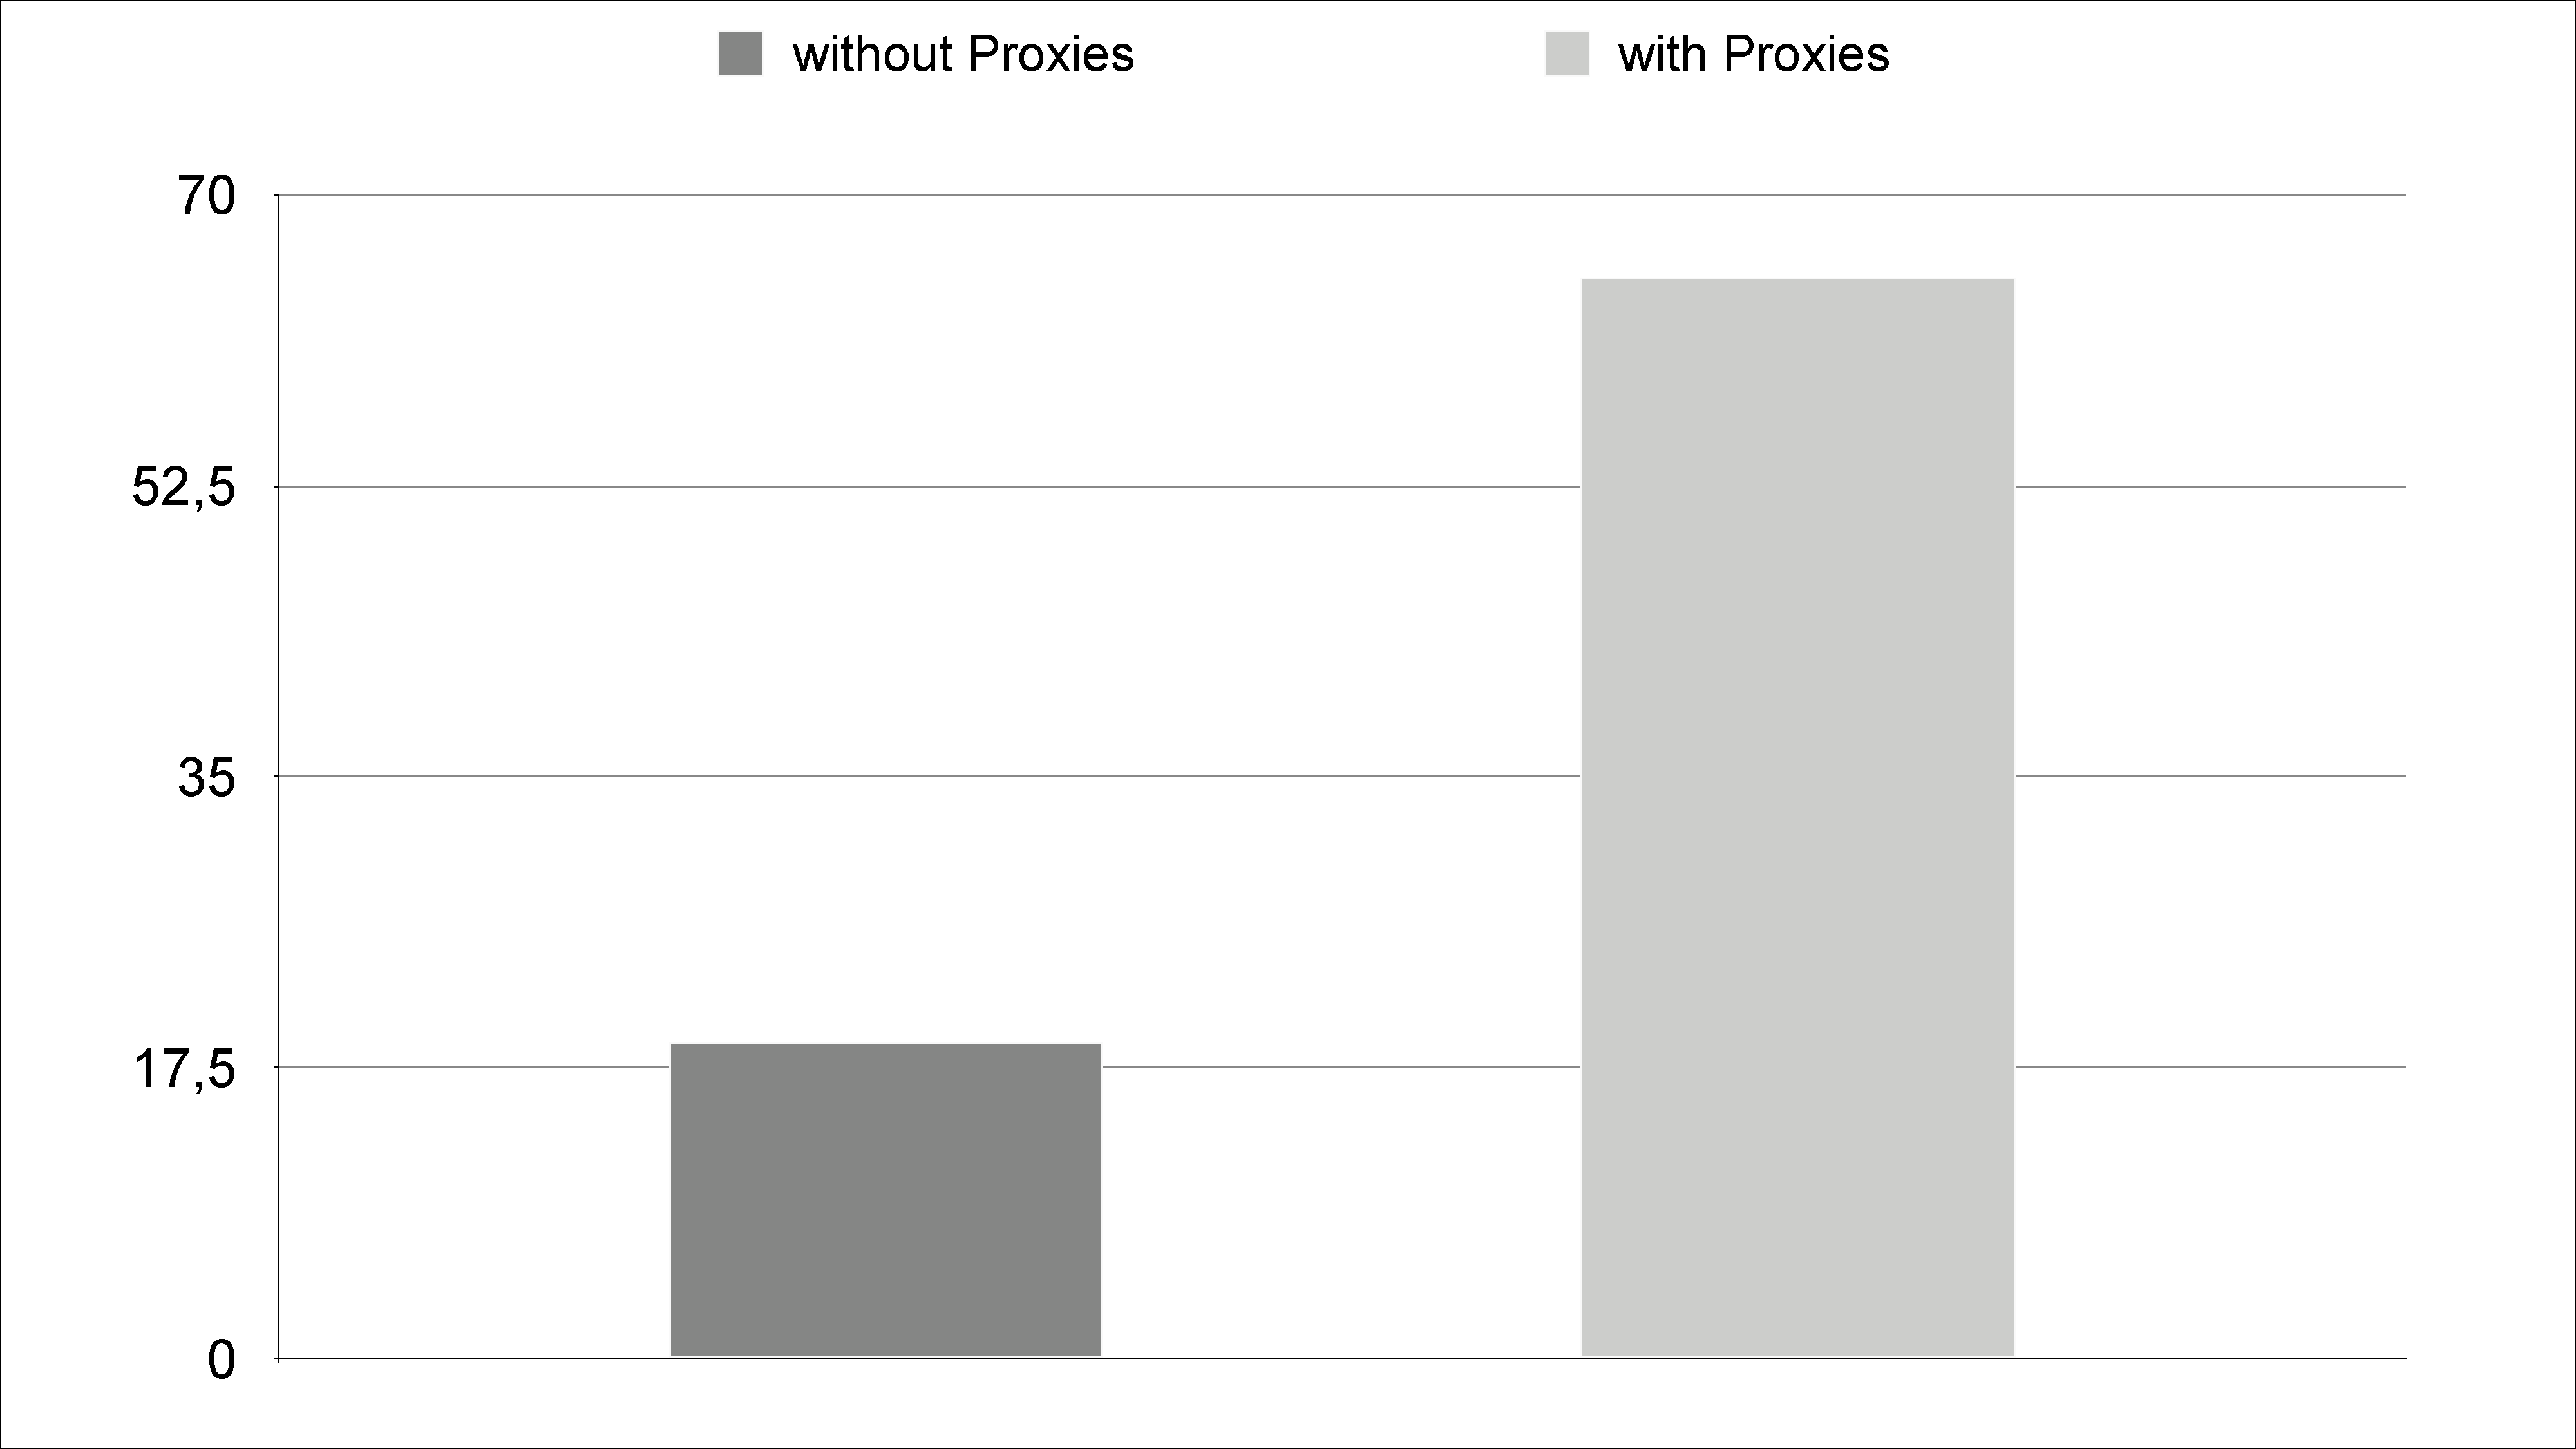
\includegraphics[width=\textwidth]{figures/memoryOverhead.pdf}
    \caption{Memory consumption when starting an empty Lively Kernel world in megabyte.}
    \label{fig:MemoryOverhead}
\end{figure}

In contrast to the memory overhead for the version-aware references, the memory consumption for different versions of the runtime does not increase linearly with the number of proxied objects or even with the number of versions:
Our implementation does not copy all objects for each version, but only creates copies when objects change between versions, effectively storing only diffs on the granularity of objects.
Therefore, the memory required for new versions of the runtime depends on how many objects change and how big those objects are.
It is, subsequentely, not possible to present this memory overhead independent of concrete usage scenarios.


\subsection{Execution Overhead}

In general, the experienced slow down is independent of the number of versions available for the system, but dependent on how many version-aware references have to be resolved during the execution of particular code.
As versions of objects are created only when objects change between versions, preserving a version of the runtime happens incrementally and not at a single moment in time.
Additionally, changing a version also does not take any relevant time as the version-aware references are not updated, but dynamically delegate differently the next time they are resolved.

To give an impression on how our implementation of object versioning impacts the execution speed, we compared using the proxies to not using the proxies for both the Octane benchmark suite and a few particular typical user interactions in Lively.
Additionally, a microbenchmark shows how much more time is necessary to resolve a single proxy-based version-aware reference.

Figure~\ref{fig:ExecutionOverhead} shows how much more time the Octane benchmarks\footnote{Note: We reduced the input size to the Splay benchmark by an order of magnitude to prevent the browser from prompting for user input during the benchmarks execution. This prompt is a reaction to the long time required to run the benchmark, cannot be disabled beforehand, and would influence the benchmark result.} take when their source is transformed before execution and references are, therefore, version-aware.
Executing the benchmarks takes between 90 and 405 times longer with version-aware references than without.
On average the slowdown is 187.5 times.

\begin{figure}[h]
    \centering
    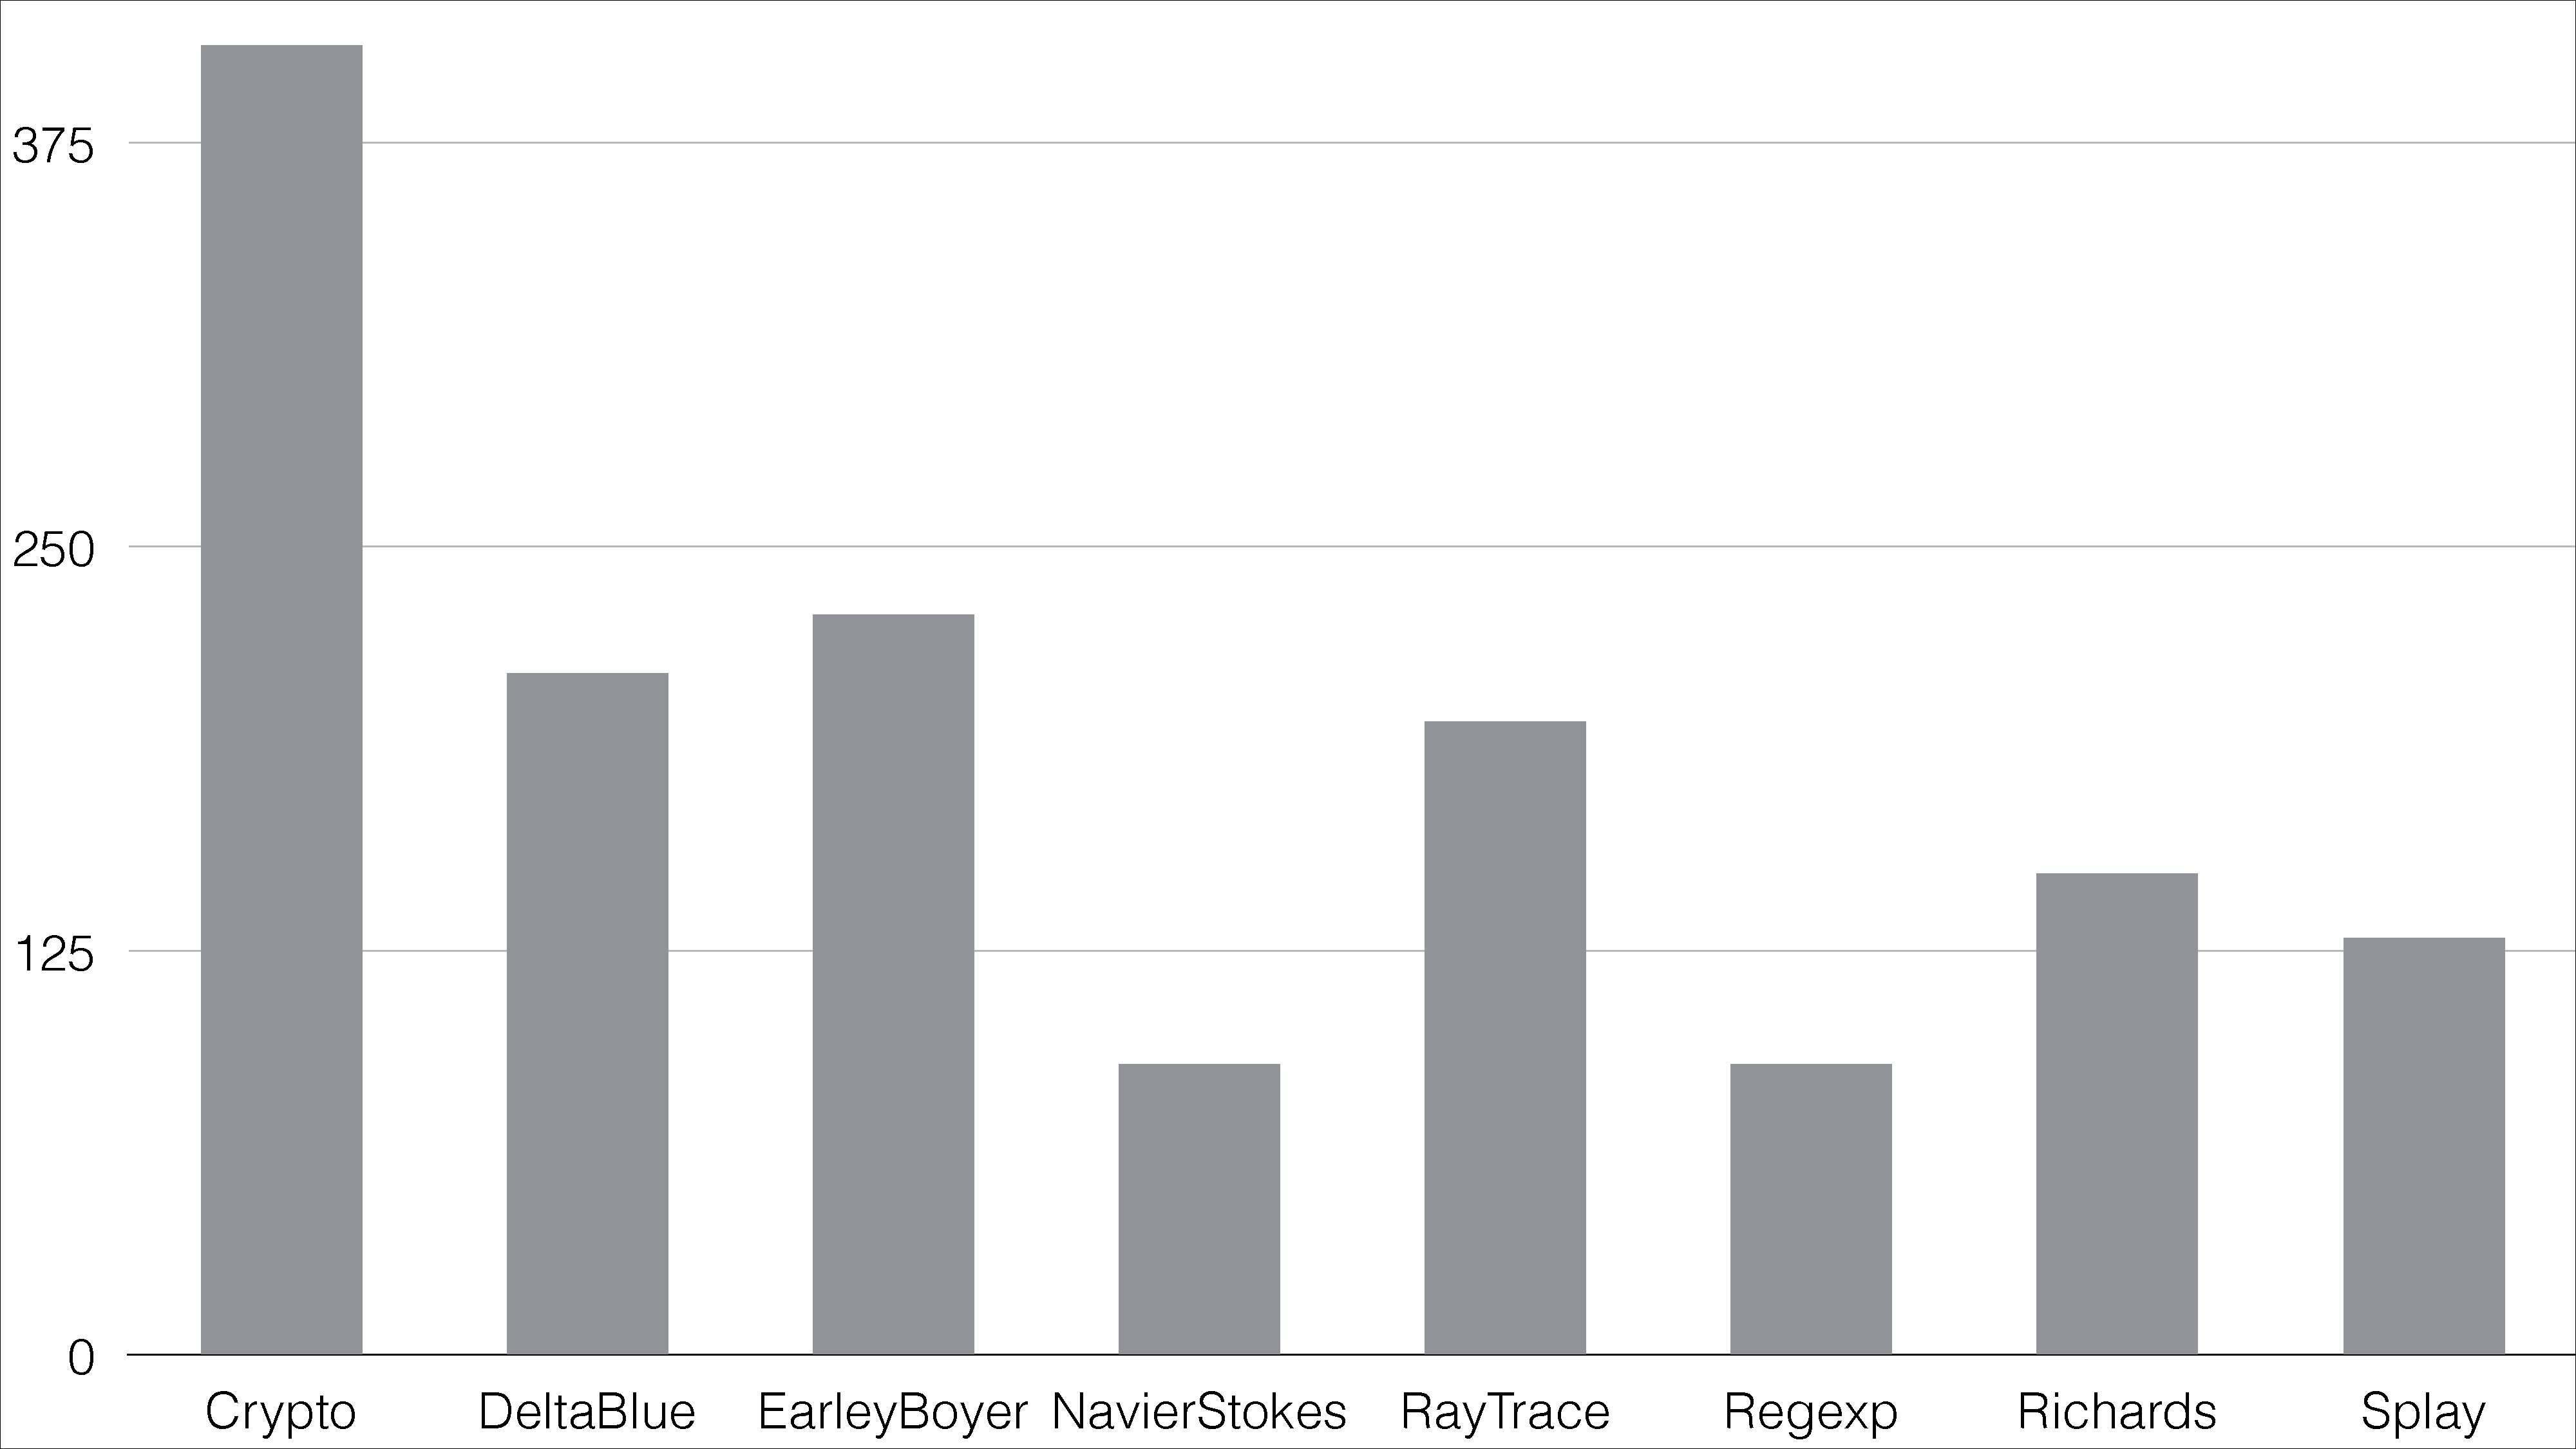
\includegraphics[width=\textwidth]{figures/executionOverhead.pdf}
    \caption{Execution overhead for proxy-based version-aware references in 100\% overhead compared to ordinary JavaScript references.}
    \label{fig:ExecutionOverhead}
\end{figure}

\todo{maybe show the execution overhead differently as it might be hard to understand that the unit is 100\% overhead and that like 2 means twice the time is necessary.. and that, therefore, each bar compares with-versioning to original performance..}

While object versioning could be used to implement application-specific undo and redo, it is primalary itented to support development and similar explorative tasks.
That could, conceivably, be an argument for providing object versioning only during development and not when programs should run at full speed.
However, besides having the disadvantage of introducing distinct usage modes, this still requires the version-aware references to resolve fast enough to not impede development significantly.

Therefore, in addition to measuring the execution of general JavaScript programs, we also timed typical user interactions in Lively.
Figure \ref{fig:LivelyInteractionsOverhead} shows a direct comparison between using proxies and not using proxies for three selected user interactions: bringing up the halo buttons on a particular morph, opening the world's menu, and opening a new System Code Browser.
The three presented interactions are among the most obviously slowed interactions compared to, for example, interactions that are more interactive or browser-supported such as dragging a morph around.
All three interaction trigger code from multiple different modules, including event handling code, rendering code, and tool-specific code.

\begin{figure}[h]
    \centering
    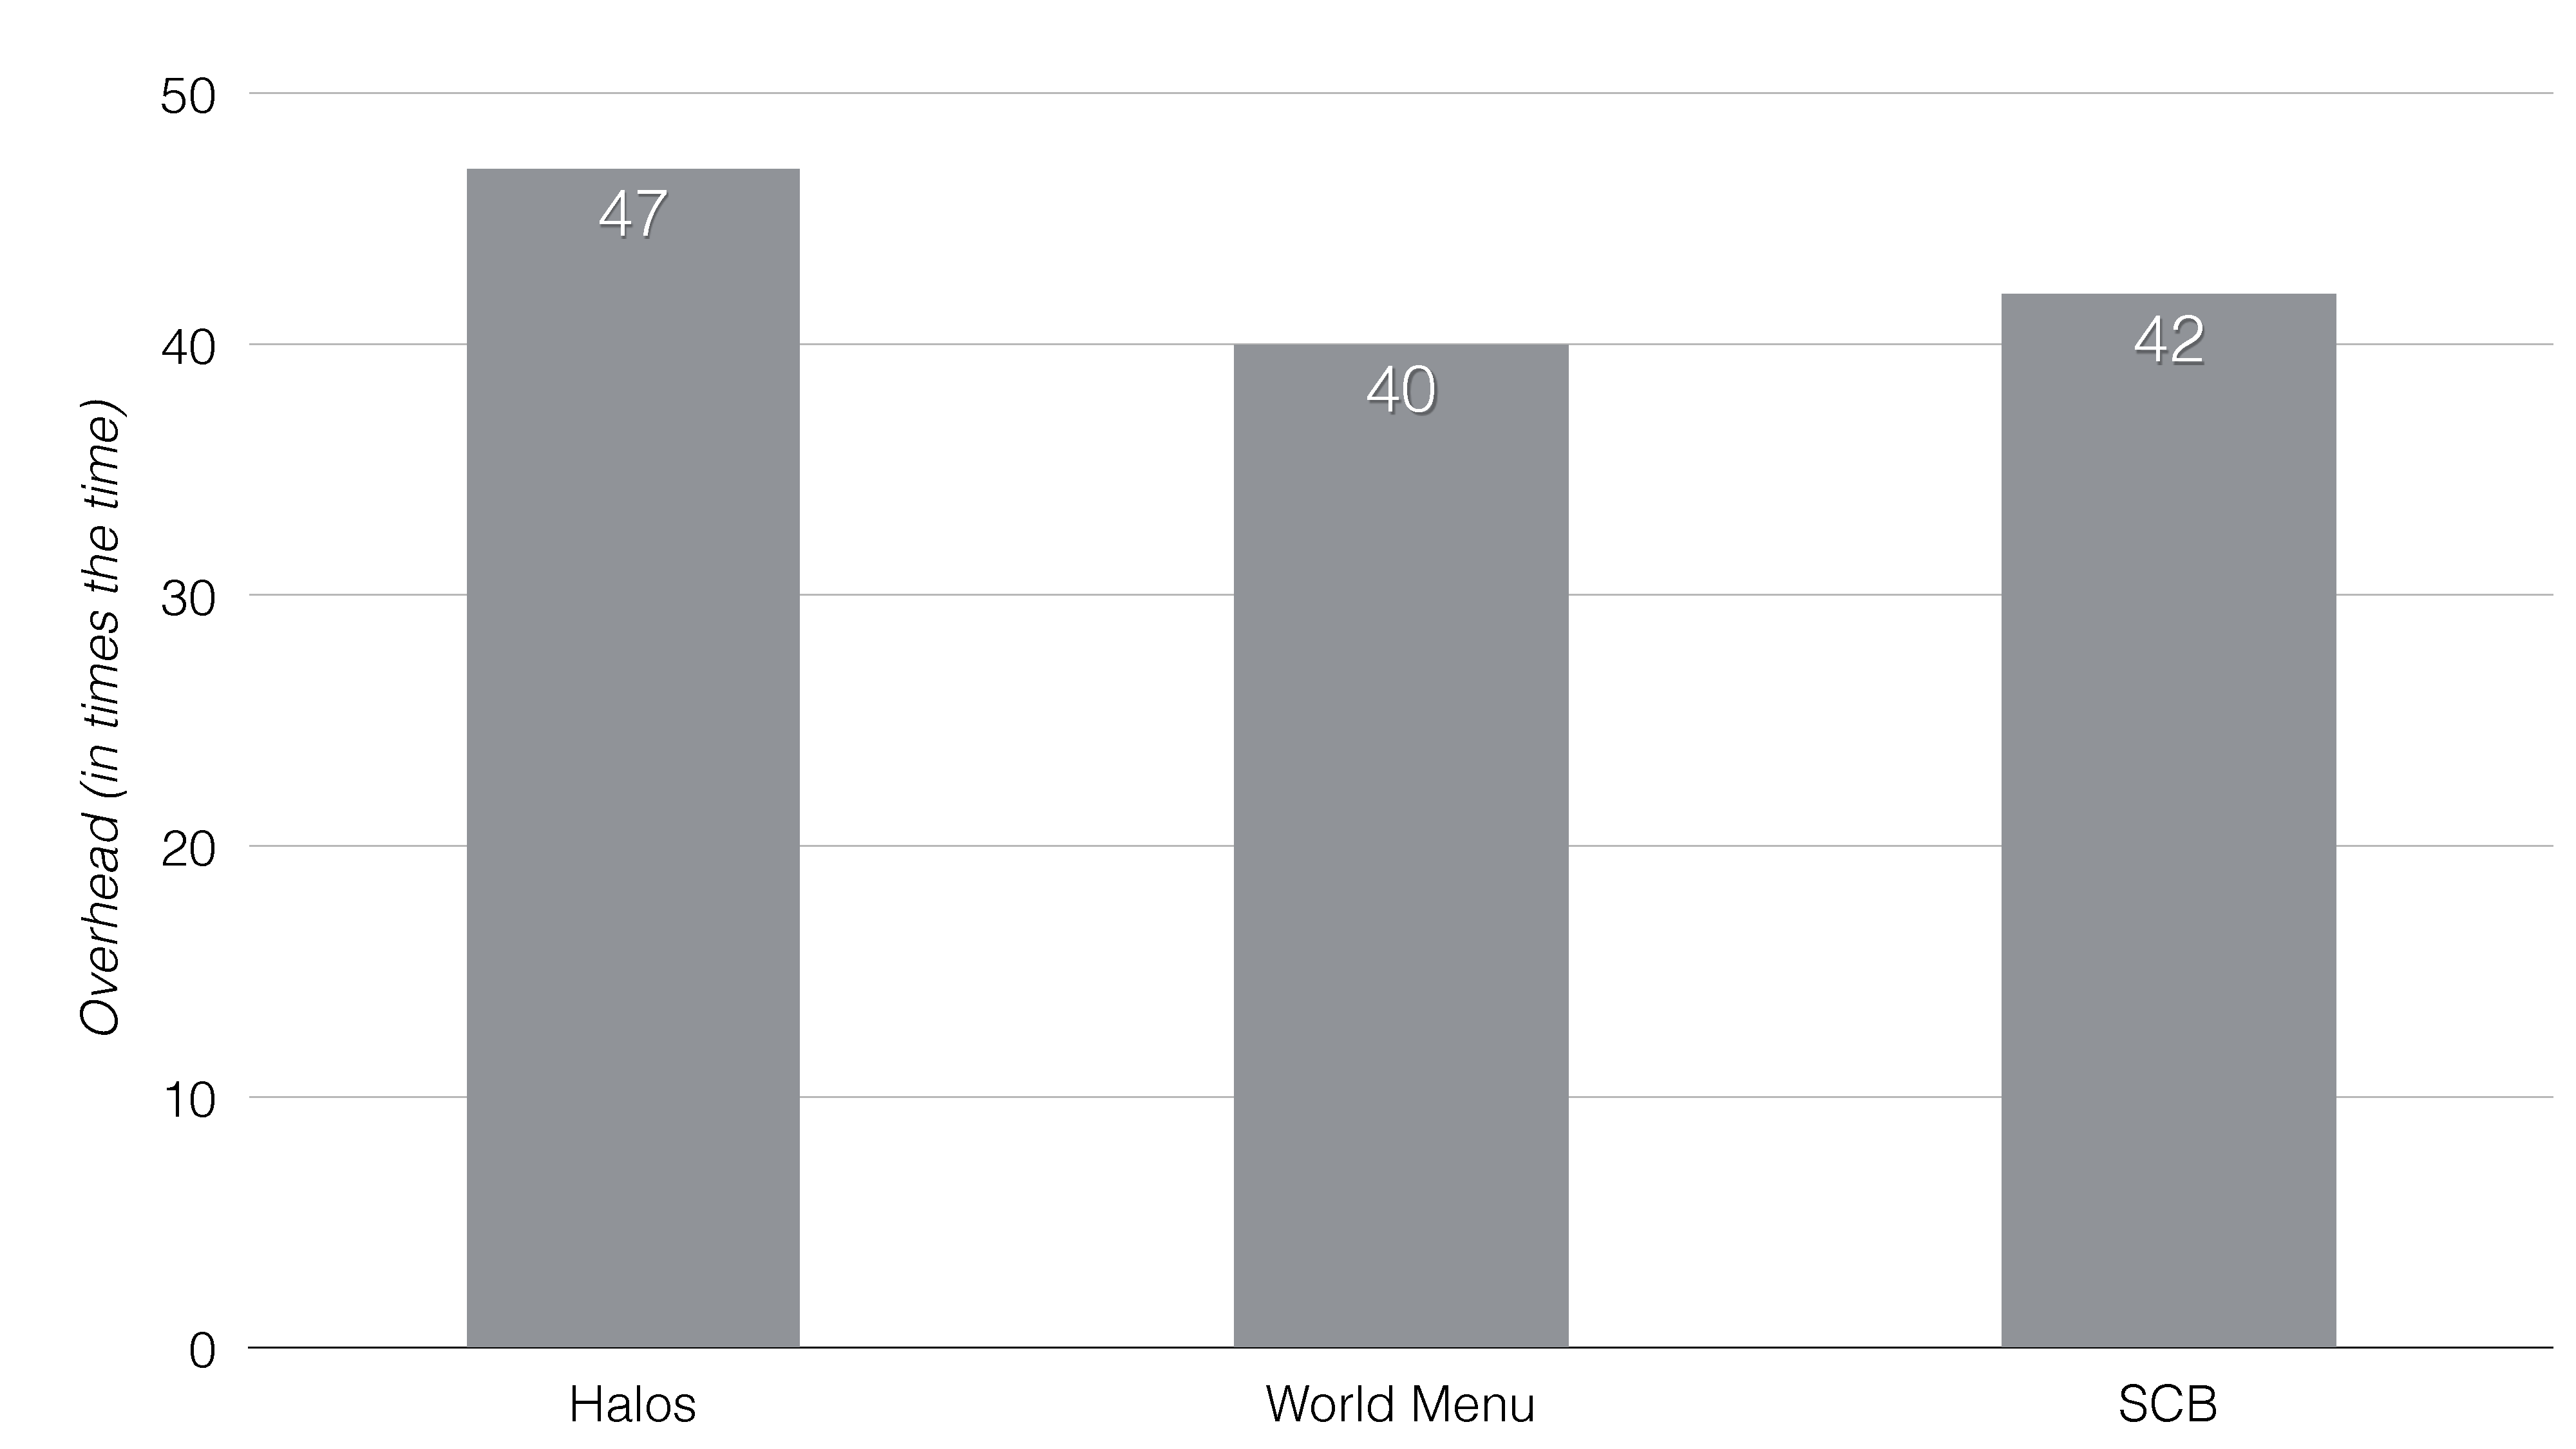
\includegraphics[width=\textwidth]{figures/livelyInteractionsOverhead.pdf}
    \caption{Execution overhead for selected user interactions in Lively in 100\% overhead.}
    \label{fig:LivelyInteractionsOverhead}
\end{figure}

Another performance related question specific to Lively is how long it takes to load a world.
This includes requesting all required modules from Lively's server, but also client-side code to resolve dependencies among modules, evaluating all loaded modules, and deserializing a Lively world.
In addition, in case version-aware references should be used, all required modules also need to be transformed.
The difference between providing object versioning and not is here a factor of around eight for loading a world: instead of around 4 seconds, the bootstrap takes around 32 seconds.

In summary, the current implementation slows down the JavaScript execution considerably: the benchmark programs need two to three orders of magnitude more time to finish, while particular typical user interactions in Lively also take two orders of magnitude more time.
As this slowdown is due to the proxy-based version-aware references, we also implemented microbenchmarks to analyze exactly how long it takes to resolve such a reference.
When two objects are either connected by a proxy-based version-aware or a direct reference and this connection is resolved a million times to call a simple function, the microbenchmark using our version-aware references takes three orders of magnitude more time: instead of on average ten milliseconds the test requires on average about 11000 milliseconds.
When we exchange the proxy-based version-aware reference for this benchmark with just a proxy---a proxy prodiving the default proxy behavior and not our versioning behavior---the difference is an order of magnitude less: using a direct reference still results in around 10 milliseconds, while placing a proxy in-between both objects results in on avg close to 2000 milliseconds.
That is, even without our specific proxy behavior, the proxies slow down the microbenchmark close to 200 times.

As explained in Section \todo{section for harmony shim proxies..}, the proxies are currently implemented using a shim library that relies on an implementation of a previous, deprecated draft of the proxy specification.
The proxies are also part of a EcmaScript specification that has not yet been finalized and completely implemented.
Further, similar indirections of object access as the default proxy handler provide could also be implemented in JavaScript.
Instead of using a proxy for an object, we could still refer only to a stand-in, but implement the proxy behavior in an ordinary JavaScript function to which we would transform the source code: instead of \lstinline{obj.prop} we could execute something similar to \lstinline{get(obj, \"name\")}, where \lstinline{get} could implement the behavior previously implemented by respective the proxy trap.
Measuring the performance of such a manually provided indirection reveals a much lower performance decrease for the previously described benchmark setup.
In fact, such an indirection would only take twice the time to read a property from a specific target in such a \lstinline{get}-function compared to reading a property directly. 
All this suggests that the performance of EcmaScript 6 Direct Proxies in Chrome might improve in the future.
At the same time, as suggested in Section \todo{future work, source transformation section}, we might also decide to base our version-aware references on source transformations and custom indirections instead of proxies altogether.

\todo{another performance related question to discuss would be whether copy-on-write on changes in new versions impedes the responsiveness of the Lively tools much..}
